\section{Introdução}
\label{sec:intro}
Um modelo eficiente de fluxo de trabalho e versionamento é muito importante para o bom desenvolvimento de um projeto de software, já que um dos principais problemas conhecidos do desenvolvimento e manutenção de software é o fenômeno denominado pelo termo "dependency hell". Este fenômeno acontece devido aos projetos de software possuírem dependências diretas e transitivas (dependências de dependências) que na verdade, nada mais são do que outros componentes de softwares que evoluem de forma independente cada qual com seu ciclo de vida e sua equipe. Assim sendo, quanto mais dependências um projeto possui, maior a probabilidade de ocorrerem conflitos entre elas.

Vincent Driessen propôs um modelo eficiente de fluxo de trabalho chamado Git-Flow ~\cite{gitflow} porém, tal modelo pode vir a ser complexo para equipes pouco entrosadas ou pouco experientes ao trabalhar com sistema de controle de versões distribuído dado uma quantidade grande de branches que tal modelo propõe. No modelo de Driessen, temos um branch para desenvolvimento do projeto, outros temporários para cada nova funcionalidade desenvolvida, um branch para release, o branch master (principal) que é usado somente para manter as versões finais com suas respectivas tags e um branch somente para os hotfixes.
Por meio deste artigo proponho uma maneira mais simples de fluxo de trabalho que acredito funcionar melhor em tais cenários e com bom aproveitamento de projetos desenvolvidos sob metodologia SCRUM~\cite{scrum} e implementados utilizando a ferramenta de gerenciamento de ciclo de vida Maven. Uma outra boa premissa também é o uso de um modelo de versionamento sugerido pela equipe de Tom Preston-Werner, cofundador do GitHub chamado Versionamento Semântico~\cite{semver} sob a licença Creative Commons como pode ser visto na figura \ref{fig:modelogitflow}

\begin{figure}[h!]
\centering
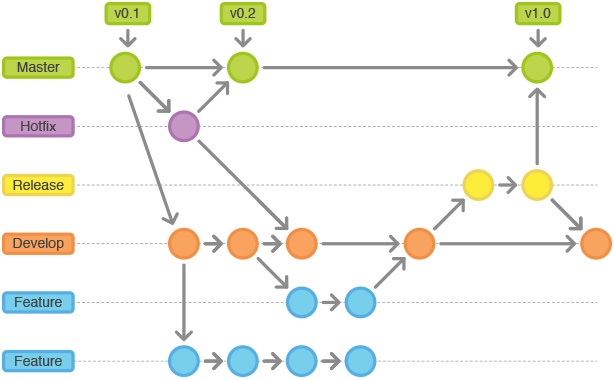
\includegraphics[width=0.7\linewidth]{img/modelo_gitflow}
\caption[Modelo de Branching GitFlow]{Modelo de branching proposto por Vincent Driessen e usado no GitFlow}
\label{fig:modelogitflow}
\end{figure}

O Versionamento Semântico padroniza a nomenclatura de versionamento de código utilizando no mínimo três conjuntos de números onde a versão do projeto é composto pela "versão maior"."versão menor"."versão de correção", sendo que a versão maior é incrementada quando se tem mudanças incompatíveis na API, a versão menor quando são adicionadas funcionalidades mantendo-se a compatibilidade da API e a versão de correção para correção de defeitos somente. Classificadores também podem ser aplicados após a versão de correção, dentre outros detalhes da nomenclatura presente em sua especificação.
\\\\
Por exemplo:
\\\\
Projeto \textbf{FrameworkTeste} na versão:\textbf{ 1.2.3-SNAPSHOT} desenvolvido sob metodologia SCRUM:
\\\\
Assim sendo, podemos condiderar:
\\\\
\textbf{Versão Maior:} 1 - Primeira especificação da API.\\
\textbf{Versão Menor:} 2 - Segundo conjunto de funcionalidades (muitas vezes associadas \~a segunda Sprint).\\
\textbf{Versão de Correção:} 3 - Esta versão geralmente é incrementada várias vezes dentro de uma mesma Sprint).\\

No modelo proposto, sugiro o Git como referência de sistema de controle de versões dado o seu funcionamento distribuído, simplicidade de alternância entre diferentes branches e facilidade de reintegração de código (merge) e será usado como referência para este artigo porém pode ser aplicado em qualquer SCM (Source Control Management). Utilizaremos também os classificadores (sufixos) adotados pelo Maven para diferenciar o projeto em estado de desenvolvimento (sufixo \textbf{-SNAPSHOT}) e estado de produto final (sem sufixo).
